\section {色彩管理}

-
    \begin{center}
        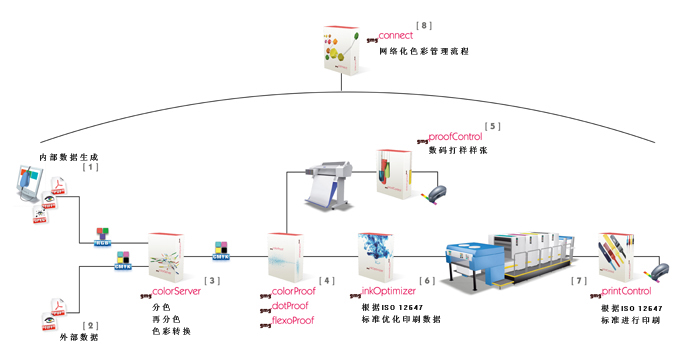
\includegraphics[scale=0.7] {colormanage.jpg}
    \end{center}

    所谓色彩管理,是指运用软、硬件结合的方法,在生产系统中自动统一地管理和调整颜色,以保证在整个过程中颜色的一致性。

    色彩管理(Color Management)是一种用于在各种数字图像设备(如扫描仪、数码相机、显示器、打印机等)之间进行可控的色彩转换的技术。色彩管理的首要目的是让不同的设备能保持相对统一的色彩表现效果。ICC制定了一套通用文件规范用于在不同操作系统和软件之间进行跨平台的色彩管理。

\subsection {色彩管理系统(CMS)的内容}

    色彩管理系统(CMS)的目的,就是通过对所有设备的管理、补偿和控制这些设备间的差别,以得到精确的可预测的色彩,一个色彩管理系统应该包括以下几部分:

    \begin{enumerate}
        \item  一个色彩匹配处理程序,即色彩管理模块(CMM);
        \item  一个与设备无关的色彩空间,通常叫做参考色彩空间或特性文件连接空间,在转换过程中起着连接的作用;
        \item  设备特性文件。设备特性化是用以界定输入设备可辨识的色域范围与输出设备可复制的色域范围的工作,并将不同设备之间RGB或CMYK的色彩与CIE所制定的设备色彩建立设备色彩与设备独立色彩间的色彩转换对应文件,该文件被称为设备特性文件。
    \end{enumerate}

    在图像链的各个环节中,校准所有的输入/输出设备,以便达到这样的目标——在与所用设备无关的情况下,总能得到期望获得的色彩再现。

    我们常常碰到这样的情况:
    \begin{itemize}
        \item  扫描结果与原稿始终有很大差别
        \item  屏幕显示的颜色和数字打样机打印出来的结果不同
        \item  数字打样机打印与印刷结果不一致
        \item  RGB图挡转成CMYK输出后颜色不一致
        \item  不同的计算机显示同一文件时颜色不一致
    \end{itemize}

    实际上,色彩管理在现代化数字印前制版系统和数字印刷领域的作用是不可忽视的。目前,很多现代化印刷生产企业在使用色彩管理以后,生产效率大大提高,同时出错率也相应减小。到底我们引入色彩管理的作用是什么呢?总结起来有以下几点:

    \begin{enumerate}
        \item  校正、制作特性文件之后,所有的设备都会达到相当一致的颜色
        \item  显示器的颜色和原稿一样
        \item  屏幕软打样(模拟印刷颜色)
        \item  数码打样
        \item  输出后的颜色会和原稿非常相近
    \end{enumerate}

\subsection {实现方式}

    \subsubsection {目的和限制}

        色彩管理的目标是在目标设备或物料上提供相对于原件最理想的色彩效果,如显示器的色彩管理。或是让用户能预览原件在不同的设备或者物料上的色彩效果,如印前在显示器上模拟印刷后的颜色等。由于不同的设备和物料的固有特性,在绝大多数情况下通过色彩管理是无法得到与原件100\%相同的色彩表现效果的。因此色彩管理的校准效果是相对的而不是绝对的。

    \subsubsection {过程}

        色彩管理的过程主要分为三个主要步骤,合称3C。
        \begin{itemize}
            \item  设备校准(Calibration)
            \item  特性化(Characterization)
            \item  色彩转换(Conversion)
        \end{itemize}

        设备校准主要是进行灰阶校准(Linearization)以抵消设备本身的伽马校正(Gamma Correction)的影响。
    特性指的是设备的色彩表现能力,通称色彩范围(色域)(Gamut)色彩输入和输出仪器以及各类彩色物料(例如油墨、显示器的发光剂和滤光片等)都有一定的色域。特性化过程对设备和物料进行相对于标准色彩空间(如sRGB)的比较测量,并以数学方式记录(Profiling)受测设备的特性,生成设备特性档案,通常是ICC色彩特性文件,以便进行色彩转换。

        色彩转换将原件的色彩根据之前的ICC色彩特性文件进行转换,也叫色域转换(Gamut Mapping)以求在目标设备或物料上提供最理想的色彩效果。

\subsection {色彩测量仪器}

    色彩测量仪器是用于测量物体的下列参数中的一种或多种数值的光学仪器:
        \begin{itemize}
            \item  反射率(Reflectance)
            \item  透射率(Transmittance)
            \item  CIE色度值(如XYZ值)
            \item  可见光谱(380nm-730nm)
            \item  辐射亮度(Spectral Radiance)
        \end{itemize}

    按原理分类,色彩测量仪器包括但不限于以下种类:

        \begin{itemize}
            \item  色温表(Color Temperature meter)
            \item  测光表(Exposure meter)
            \item  浓度计(Densitometer)
            \item  色度计(Colorimeter)
            \item  光谱光度计(Spectrophotometer)(也称作分光仪)
            \item  光谱辐射计(Spectroradiometer)
        \end{itemize}

    其中色度计常见于业余的显示器校准,这类仪器通过内部红绿蓝滤光片来测得RGB的刺激值,结构简单,价格相对低廉。色度计有滤光片老化后失准、无法准确测量宽色域显示器等缺陷。分光仪通过测量物体表面反射光的光谱来获取读数,比色度计准确且适用范围更为广泛。分光仪的技术较为复杂,价格高昂。有分球式分光光度计、多角度分光光度计(用于求得镜面反射的物品颜色)等。

    按用途分类,色彩测量仪器根据用途可被分为三大类:

    \begin{itemize}
        \item  用于测量光源色(Self-Luminance or Emission),测量对象本身发光,如显示器和灯具。
        \item  用于测量反射稿(Surface Color),测量对象本身不发光,通过反射其他光源发生颜色。如印刷品、打印机。
        \item  用于测量透射稿(Transmitted Color),测量对象是透光的,如胶片。
    \end{itemize}

\subsection {色彩管理过程}

    色彩管理分为校准测量环节、操作系统环节和应用软件环节。

    \subsubsection {校准和测量}

    校准仪器和进行色彩管理需要专门的软件,测量软件的读取方式和算法对测量的精度影响极大。市面上的色彩校准仪器一般自带有简易的配套软件,但通常功能有诸多限制,测量精度也不高。专业级的商业颜色管理软件价格高昂。在开源软件中Argyll CMS配合其图形化前端dispcalGUI能实现专业级的设备校准和色彩管理。

    \subsubsection {操作系统}

    一般来说在设备的操作系统中加载ICC色彩特性文件后,操作系统会按照其中信息将源图像的信息转换成匹配目标设备显示特性的状态。主流的操作系统如Microsoft Windows、Mac OS X和GNU/Linux等都已经内置了对ICC规范的支持。

    \subsubsection {应用软件}

    图像处理系统如Adobe Photoshop和GIMP为了在不同的显示器和打印输出设备上保持色彩的一致性也内置了独立于操作系统以外的色彩管理模块,通过模拟目标设备的色彩空间的显示来保证编辑时的色彩能在目标设备上得到理想的效果。Mozilla Firefox和Safari等网络浏览器也带有类似的功能。


    一个理想的色彩管理过程如下所述:

    \begin{enumerate}
        \item  确定显示器的颜色性能特点:有些色彩管理系统将各个厂家提供的显示器颜色描述文件(Profile)预置在一起,构成一个全面的内部预置文件概况库,在确定显示器的颜色特性时调用即可。
        \item  校准显示器。将显示器的白点及其它显示特性调整到符合你的输出要求。例如,如果输出到印刷介质的话,那么可以考虑将显示器的白点校准到印刷纸的色温。
        \item  确定扫描仪或其它输入设备的特性。如果色彩管理系统提供一个IT8样本,就可对它进行扫描或拍摄。然后将所得颜色数值与标准颜色数值进行比较,将所有差异信息作为扫描仪的Profile文件记录下来,以备扫描时使用。
        \item  颜色管理系统将扫描结果转换为显示器的颜色空间。
        \item  确定颜色打印及输出设备的特性。即为色彩管理系统所支持的彩色打印机,印刷条件及其它输出设备选择一个颜色特征描述文件。
        \item  颜色管理系统利用显示器和印刷机的概况文件去变换颜色,有些系统允许在屏幕上进行“软打样”(即在屏幕上表示CMYK颜色)。
    \end{enumerate}

    显示器虽然是一个计算机输出设备,但对设计人员来说,它却是调节颜色、进行颜色搭配、观察图像深浅、进行层次调节的一个重要参考窗口。虽然我们都知道显示器上的颜色和印刷出来的颜色有差距,但对图像的层次、深浅,清晰度等方面的判断都是依据显示器的显示而来的,因为我们不可能对每一个像素的颜色数据都去判读。其次,显示器是设计时的视觉中心,不管图像的色彩模式是什么,都要反映到显示器上来。RGB色彩模式的数字图像要显示器表现,CMYK色彩模式的数字图像也要经转换在显示器上显示出来,同一文件的这两种色彩模式的图像可能在显示器上的颜色会有差别。

\subsection { ICC色彩管理}

    \subsubsection { ICC简介}

        在印刷工作流程中,涉及到许多图像设备,比如数码相机、扫描仪、打印机、数码打样机、印刷机和显示器等,但是对于其中的每一种设备,都有不同的色彩表现能力。例如,一个显示器中一个数值为R=128, G=128, B=128 的像素点,应该产生一个完全的中性灰色调,但是在一些显示设备上,这个灰看起来偏暖,也就是发红,或者在另外一显示些设备上,这个灰看起来偏冷,也就是发蓝。设备的这些固有特性使一幅图像从一个设备传到到另一个设备上的时候,图像色彩的一致性,准确性和可预见性都很难保证。

    \begin{center}
        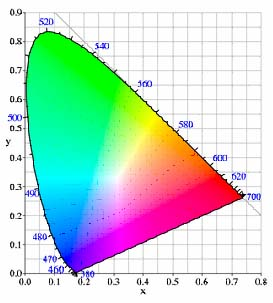
\includegraphics[scale=0.7] {icc.jpg}
    \end{center}

        国际色彩联盟(ICC)的成立就是为了解决这个问题。在 1993 年由苹果电脑和其它7家公司创立了ICC,现在ICC有超过70家设备制造商和软件开发商成员,包括 SONY,HP,Creo,Adobe 和 Quark 等。其作用就是创建色彩管理的标准和核心文件的标准格式。所努力开发的核心就是 ICC Profile(ICC 色彩特性文件)和色彩管理模块(CMM)。这两者保证了色彩在不同应用程序,不同电脑平台,不同图像设备之间传递的一致性。

    \subsubsection { ICC Profile}

        色彩管理的基础就是 ICC Profile,它是一种跨平台的文件格式,它定义了色彩在不同设备或不同色彩空间上进行匹配所需要的色彩数据。每一个 ICC Profile 文件至少包含一对核心数据:

        \begin{itemize}
            \item  设备相关的色彩数据(例如,该设备独有的RGB色彩显示数据);
            \item  根据设备相关的数据而得到的与设备无关的色彩数据。
            \item  与设备无关的色彩数据,也被称为 Profile 联接空间(PCS)。
        \end{itemize}

        一些设备的 Profile 文件,如扫描仪的 Profile,只有一个设备到 PCS 的色彩数据转换表,因为对于扫描仪来说,只是通过它产生颜色并输出到其它设备中。而对于另外一些设备,比如印刷机的 Profile,就需要包括一个设备到 PCS 的色彩数据转换表和 PCS 到印刷机的色彩数据转换表。

    \subsubsection { 色彩与设备无关}

        色彩与设备无关是实现图像信息交换标准的重要一环,其含义为某一种图像处理设备所处理获得的图像色彩数据结果,在另一种处理设备上应该能够得到相应的还原。要实现色彩与设备无关,首先必须能够客观地评价图像的颜色和密度与处理设备之间的变换特性。

        用来创建颜色的设备包括扫描仪、显示器、桌面打印机、打样设备和印刷机,每种设备都可再现一个有限的颜色范围。我们把一个设备能再现的颜色称为色表,很多设备的色表被记录在一个称为“Profile”的文件中,色彩管理系统就是从这个文件中获取该设备的色表。色彩管理系统将把某个设备的色表转换为一个与设备无关的颜色模式CIE Lab颜色模式,然后进行设备间的颜色映射处理,将转换后的与设备无关的颜色信息嵌入到另一个设备的色表中,从而使设备的色表能对应起来。有两种协调不同设备的色谱的方法:一种方法是通过将所有的颜色变换到设备的色谱中,从而保留颜色间的关系;另一种方法是映射色谱之外的颜色到设备能产生的颜色中,而不保留颜色间的关系。

\subsection { 色彩管理的好处}

        通过高效的,可预知的,成熟的色彩管理,可增强专业设计的能力,更好的实现“所见即所得”。将会为客户带来以下好处:
    \begin{enumerate}
        \item  与预期颜色准确匹配;
        \item  使用不同设备在不同时间,不同介质上实现色彩的一致性;
        \item  实现与客户更好的合作;
        \item  缩短生产周期,降低返工率;
        \item  降低生产成本,提高工作效率;
        \item  提高客户满意度,提升产品的质量;
        \item  可以使在显示器或数码打样机打印的数码稿上看到的颜色与最终印刷品的颜色达到完全一致。
    \end{enumerate}
